\documentclass[conference]{IEEEtran}

\usepackage{float}
\usepackage[pdftex]{graphicx}
\graphicspath{ {pictures/}{../pdf/}{../jpeg/} }
\DeclareGraphicsExtensions{.pdf,.jpeg,.png,.PNG}

% *** SUBFig PACKAGES ***
\ifCLASSOPTIONcompsoc
 \usepackage[caption=false,font=normalsize,labelfont=sf,textfont=sf]{subfig}
\else
 \usepackage[caption=false,font=footnotesize]{subfig}
\fi

% correct bad hyphenation here
\hyphenation{op-tical net-works semi-conduc-tor}

% HOW TO make a command ("tab" here)
\newcommand\tab[1][0.4cm]{\hspace*{#1}}
% This line makes the collumns on the last line even
\usepackage{flushend}
\usepackage{tabularx,booktabs,textcomp}
% Additions for custom TabularX environment tables: 
\newcolumntype{C}{>{\centering\arr«aybackslash}X} % centered version of "X" type
\newcolumntype{L}{>{\raggedright\arraybackslash}X} % LEFT version... "\...right" works?
% Next three lines take [1], [2], [3], [4] and cite as [1-4]:
\usepackage[noadjust]{cite}
\renewcommand{\citepunct}{,\penalty\citepunctpenalty\,}
\renewcommand{\citedash}{--}    % optionally
% Include Smileys :) 
\usepackage{wasysym}
% Include to generate random text: 
\usepackage{lipsum} % USE: "\lipsum[1]" to generate 1 paragraph of random text 
% hyperlinks
\usepackage{hyperref}
% equations
\usepackage{amsmath}
\usepackage{amssymb}
% url on references
\usepackage{url}

% ----------------------------------

\usepackage{graphicx}
\graphicspath{ {./pictures/} }

\begin{document}

\title{Handwritten Letter Recognition\\
Research Report}


% AUTHOR
\author{\IEEEauthorblockN{Ricardo Cruz, Nº MEC: 93118\\ 
Email: ricardo.cruz29@ua.pt}
\IEEEauthorblockA{Universidade de Aveiro\\
DETI\\
Tópicos de Aprendizagem Automática\\
Teacher: Pétia Georgieva}
\and
\IEEEauthorblockN{Pedro Amaral, Nº MEC: 93283\\
Email: pedro.amaral@ua.pt}
\IEEEauthorblockA{Universidade de Aveiro\\
DETI\\
Tópicos de Aprendizagem Automática\\
Teacher: Pétia Georgieva}
}

% make the title area
\maketitle

\thispagestyle{plain}
\pagestyle{plain}

\begin{abstract}

Handwritten Letter Recognition is a deep learning classification problem that consists in recognizing handwritten capital letters, lowercase letters and numbers, from images. Handwritten Letter Recognition is required for understanding forms filled by hand. Forms for insurance, bank payments and a lot more are use cases examples where these algorithms can perform. In order to present our solution, a data set with over 3000 images was considered. In it there are variations of each letter and number to represent different variations in calligraphy.

\end{abstract}
% no keywords

\section{Introduction}

Handwritten Letter Recognition may help in a lot of real word situations. Recognizing handwritten letters and numbers helps translation of data from papers to computer. With this, time and money are saved, and this is why deep learning in general is a fast growing technology in modern days. Handwritten letters and numbers recognition is a specific real world case example where a deep learning algorithm can help. This is a area with exponentially growth that points to the future of computers. Computers that are able to understand and do the work that would take a human a lot more time is highly requested in modern days where data is getting bigger and bigger. This report explains which methods, models and techniques of deep learning were used to construct this algorithm, as well as comparisons of different models to see which one leads to better results.
\linebreak
\tab This report contains the approach to the first project of TAA - Tópicos de Aprendizagem Automática - at Universidade de Aveiro. Head teacher of this course, Pétia Georgieva, introduced us examples of deep learning problems but we decided to think of another real life examples where we could apply our knowledge. We foresee this subject to be a major area and so we decided to tackle this problem and look up about this.
\linebreak
\tab In the next sections we will start by analysing our chosen data set, then we will apply some pre-procession algorithms, followed by a description and training of 2 deep learning models and finally, we will optimize these models.


\section{Data Set Analysis}
For this project we used a data set that contains 3000+ images of handwritten letters and numbers. To see the data set used click  \href{https://www.kaggle.com/dhruvildave/english-handwritten-characters-dataset}{here}.

As this is a classification problem each image is classified as a class which may be a capital letter, lowercase letter or number. In the data set each class has associated 55 images, which contributes to the capability of the algorithm to understand calligraphy variations. Calligraphy variation is the major obstacle for this algorithm and a complete data set with a lot of examples of each class is essential to the algorithm be able to obtain high accuracy percentages. Below we can see an example of different calligraphies for the same class.

\begin{figure}[H]
    \centering
    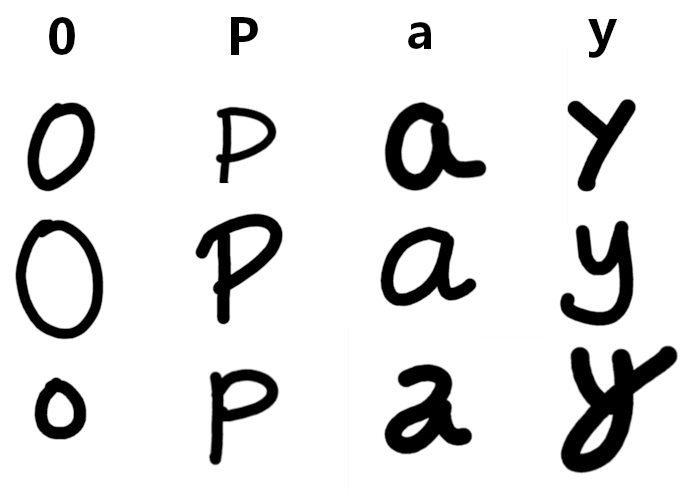
\includegraphics[width=3.5in]{pictures/4letras.png}
    \caption{Example of calligraphy variation}\label{fig:example4}
\end{figure}

We observe that for each letter and number there are slight differences that hinder the model in obtaining better results. This is the biggest problem to this algorithm and to tackle this it is necessary to have a data set with a high number of examples per class. Furthermore, it is important to have homogeneity in the data set (in other words, to have a similar number of examples in each class) preventing the existence of classes with little accuracy. In the following figure we can observe that our data set has 55 images for each class, meaning that we have an homogeneous data set and problems associated with disparity between accuracy in classes are reduced.
 
\begin{figure}[H]
    \centering
    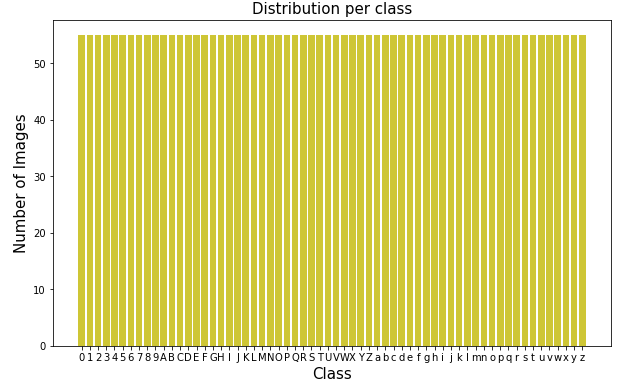
\includegraphics[width=3.5in]{pictures/DistributionOfEachClass.PNG}
    \caption{Distribution of examples per class}\label{fig:example4}
\end{figure}

Having a complete data-set is important however, it is often not enough for the algorithm to obtain good results. Besides this it is needed to have other techniques to tackle this issue. In the next section, we talk about our approach to obtain better results.

\section{Pre-processing Data}
\subsection{Description}

We stated before that we are using a data set with over 3000 images and so each image require some sort of pre-processing to increase the effectiveness of the algorithm. Data that is pre-processed in the right way is a major step for higher performances and this step should be a first approach to increase the accuracy of the algorithm. To tackle this problem we started by transforming the image from RGB(1) to grayscale(2), then we cropped it removing most of the white space(3), followed by a resizing to a fixed value(4) and finally, the image was normalized. Most of these steps can be observed in the figure below and in the next subsections there are further explanations about them.

\begin{figure}[H]
    \centering
    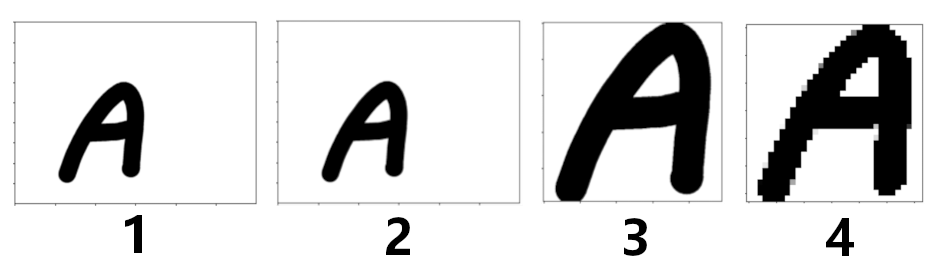
\includegraphics[width=3.5in]{pictures/pre processing.png}
    \caption{Pre-processing steps}\label{fig:example4}
\end{figure}

\subsection{Grayscaling}

The first step of preparing our data was conversion of the images to grayscale. Images that are in the data set are in RGB and this leads to a considerable larger amount of data the algorithm has to process. RBG images have 3 channels and this leads to triple the amount of the data. To put this in perspective, an image that has 50x50 pixels would have 2500 pixels to be processed and a RGB image would have 7500 pixels. This leads to considerable increases of time the algorithm takes and it is does not bring any advantage since the images were already in black and white. Even if they had more colors our images contain only numbers and letters so the color would not be a major aspect to differentiate them. Taking all of this in consideration and seeing only advantages we decided to convert our images into grayscale.

\subsection{Cropping}
The next step we decided to make was cropping our images. We obtained this idea from an article \cite{M} that applied this method to remove as much irrelevant pixels as possible. Another reason we decided to implement this method was the high variance in our model. Since one of the solutions to high variance is removing features we tried to make our images smaller which presented worse results since we could not afford more quality loss in some pictures. Therefore, removing irrelevant pixels allowed to make our images smaller while maintaining enough quality for the letter or number to be understood since they now occupy a bigger part of the picture. In the table below we can see the improvement this technique made.

\begin{table}[H]
\centering
\caption{Cropping Results}
\begin{tabular}{ | m{6em} | m{3cm} | m{3cm} | } 
\hline
 & Without Cropping & With Cropping\\ 
\hline
Test Accuracy & 0.5615835785865784 & 0.7639296054840088 \\
\hline
Test Loss & 2.1298577785491943 & 0.9568818807601929 \\
\hline
\end{tabular}
\end{table}

\subsection{Resizing}
After cropping the images from our data set we did an image resizing. This step is mandatory because all images given to our neural network need to have the same size. We decided on an image size of 32x32 pixels since this was the most common value we got from research. Although a bigger image could allow for better results since the image quality would be higher it would also take more computing power to analyse. With this process we were able to homogenize our images.

\subsection{Normalizing}
Finally as our last approach we saw that it was possible to increase the global quality of the image by normalizing it. This consists in changing the range of the pixels intensity value. This way we got a common scale and every pixel is in it range. This homogenizes and correct any issues with the images and increases their global quality leading to better recognition by the algorithm. 

\subsection{Conclusion}
In summary this sequence of steps got us better results. Pre-processing data the right way depending on the data-set is a major step to obtain better results. There were another steps in pre-processing that did not fit with our data-set. For instance data-augmentation, which consists in defining a threshold of examples for each class so that there is less difference between the number examples of each class. This step would prevent less accuracy for classes that had fewer examples comparing to others but, in our case, this step was not needed because our data-set has the same amount of examples of each class. There are other steps but doing all of them does not lead necessarily to better results, it always depends on the cost efficiency equation as well as the data-set it is being used. Despite not using every single strategy of pre-processing we were able to conclude that the steps we took were advantageous and allowed us getting into better results.


\section{ML Model Description}
As said before our theme is handwritten letter recognition and, therefore, our goal is to associate an image of a letter to that letter. As a result our data science problem is a classification problem and, from our research, the most used model for this type of problem is a Deep Convolutional Neural Network. In order to implement it in code we decided to use the library "Tensorflow" which automates some steps so that it would be faster to develop.

\subsection{Layers \cite{G}} We used 5 different types of layers building our models:

\subsubsection{Convolutional Layer} The Convolutional layer is the most important part of a convolutional neural network and allows to extract features from an image.

\subsubsection{Max Pooling Layer} The Max Pooling Layer is one of the most common pooling layers and reduces the sizes of the output of the convolutional layer being usually used together.

\subsubsection{Flattening Layer} The flattening layer converts any matrix it receives into a vector.

\subsubsection{Dense Layer} The dense layer is a neural network layer in which each of its neurons receives input from all neurons of the previous layer. This makes it so that it can also be used as an output layer.

\subsubsection{Dropout Layer} The Dropout Layer is a technique that helps preventing a model from overfitting by removing hidden units with a certain probability.

\subsection{Activation Function \cite{L} \cite{O}} All our layers with the exception of the last Dense Layer in each model (which acts as the Output Layer) use the ReLU activation function. This simple function outputs the value it received if positive and if negative it outputs 0. For the last layer we used the sigmoid activation function. This function receives a real value as an input and outputs a value in between 0 and 1.

\subsection{Loss Function \cite{Q}} Both our models use the Categorical Crossentropy loss function. The loss value resulting of this function increases as the probability the model outputs for the right class decreases.

\subsection{Optimizer \cite{R}} For our optimizer we decided to use Adam since, from our research, this algorithm combines the advantages of two others. It maintains a per-parameter learning rate (from Adaptive Gradient Algorithm) and the learning rates are obtained from the average of recent magnitudes of the gradients for the weight (from Root Mean Square Propagation).

\subsection{Model} In the next subsections we can see 2 models that we used to try to solve our problem.

\subsubsection{Model with 3 Convolutional Layers}
This model is heavily inspired in an algorithm published on "kaggle"\cite{S} where our data set is hosted and also where we started our research. It is made of 3 two-dimensional convolutional layers separated and followed by two-dimensional Max Pooling layers, 1 Flatten layer and 2 Dense Layers.

\subsubsection{Model with 2 Convolutional Layers}
This model is heavily inspired in the description of the algorithm in this article\cite{M}. It is made of 2 two-dimensional convolutional layers followed by a Max Pooling Layer, 2 Dropout Layers, 1 Flatten Layer and 3 Dense Layers.

\section{Model Training}
\subsection{Data Splitting}

In a previous section we talked about our data set and affirmed that it contains 3000+ images. In this section we explain how we split these data into different sets that have different goals. We split data into two sets - Train, Test - that as said before, have different purposes towards helping our models. Next we will explain in more detail which one of this sets as well as a more in depth analysis about their goals.
\linebreak
\tab The \textbf{Train} set consists in a set with 80\% of the original data set. This set has a considerable big percentage in comparison to the other set, because this set is the one that the model will use to train. For small data sets(less than 10000 examples) it is defined a standard distribution that consists in a share of 60\% to the training set, 20\% to the validation set and finally 20\% for to the testing set. However, as we decided to use k-fold cross validation(which will be explained below) the percentage that was assigned to the validation set was reassigned to the training set.

The \textbf{Test} set consists of the remaining 20\% of the original data set. This set is made of images that the model has never seen before and serves the purpose of testing it after the model training is complete. Even if it contains only 20\% this is a considerable sample of images, representing the calligraphy variations in approximation to real life.

\subsection{K-Fold Cross Validation \cite{A} \cite{E}}
In the previous section we introduced the concept of k-fold cross validation. Analyzing in depth this technique it can be defined as a procedure used to evaluate machine learning hyper parameters of a model on a limited data sample. In K-Fold CV the associated data set - Train set - is split into a K number of folds where each fold is used as a validation set at some point. For instance, lets imagine the scenario of 4-Fold cross validation(K=4) that was the k parameter we chose in our own project. Here, the data set is split into four folds. In the first iteration, the first fold is used to validate the model and the rest are used to train the model. In the second iteration, the second fold is used as the validation set while the rest serve as the training set. This process is repeated until each fold of the four folds have been used as the validation set. Although in the standard way the data-set being divided into 3 data sets - Train, Validation, Test - when using K-fold cross validation we do not have a specific set whose goal is to validate. Instead, the validation set changes, making it so that every fold is used to validate and training, giving rise to more realistic values, unlike the standard way in which the examples of the validation set are static, and may therefore not be realistic. It is because of this that the Train set has 80\%, also encompassing the percentage normally assigned to the validation set.

After making this process we then made some graphics to analyse the results. Therefore we can see below, for each model, the confusion matrix, the comparison between training accuracy and cross validation accuracy over the epochs, the comparison between training loss and cross validation loss over the epochs and the accuracy of each class.

\begin{figure}[H]
    \centering
    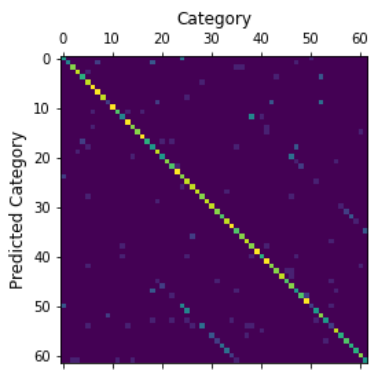
\includegraphics[width=3.5in]{pictures/model1_confmatrix.png}
    \caption{Confusion Matrix (First Model)}\label{fig:example4}
\end{figure}

\begin{figure}[H]
    \centering
    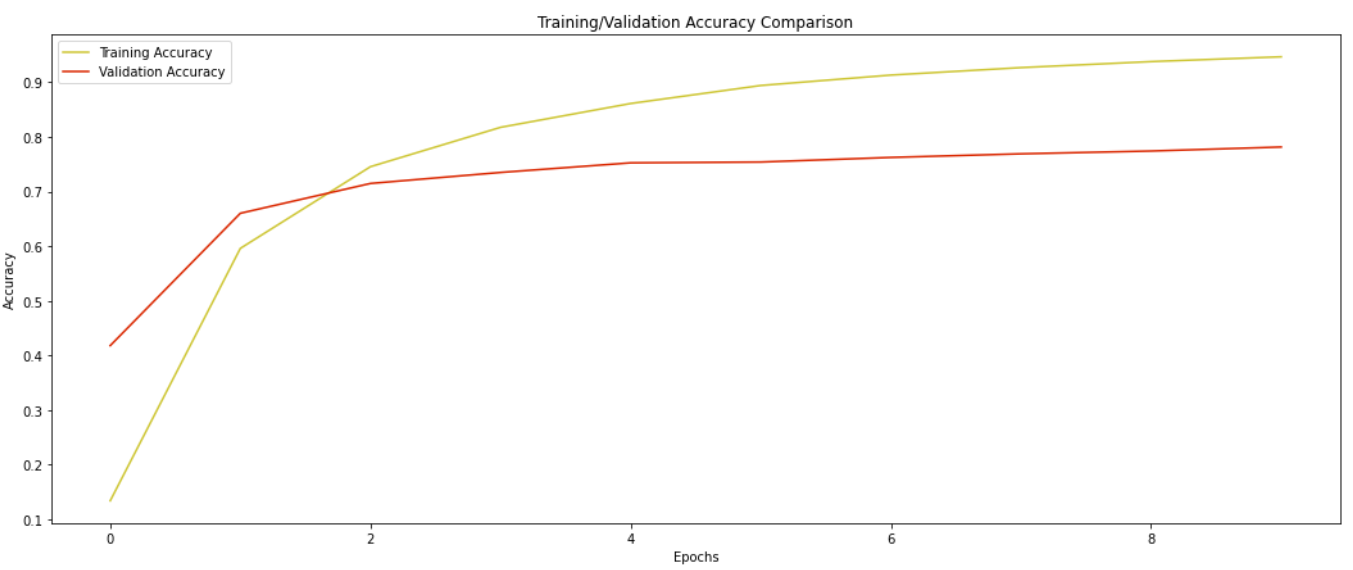
\includegraphics[width=3.5in]{pictures/model1_accuracy.png}
    \caption{Cross Validation Accuracy (First Model)}\label{fig:example4}
\end{figure}

\begin{figure}[H]
    \centering
    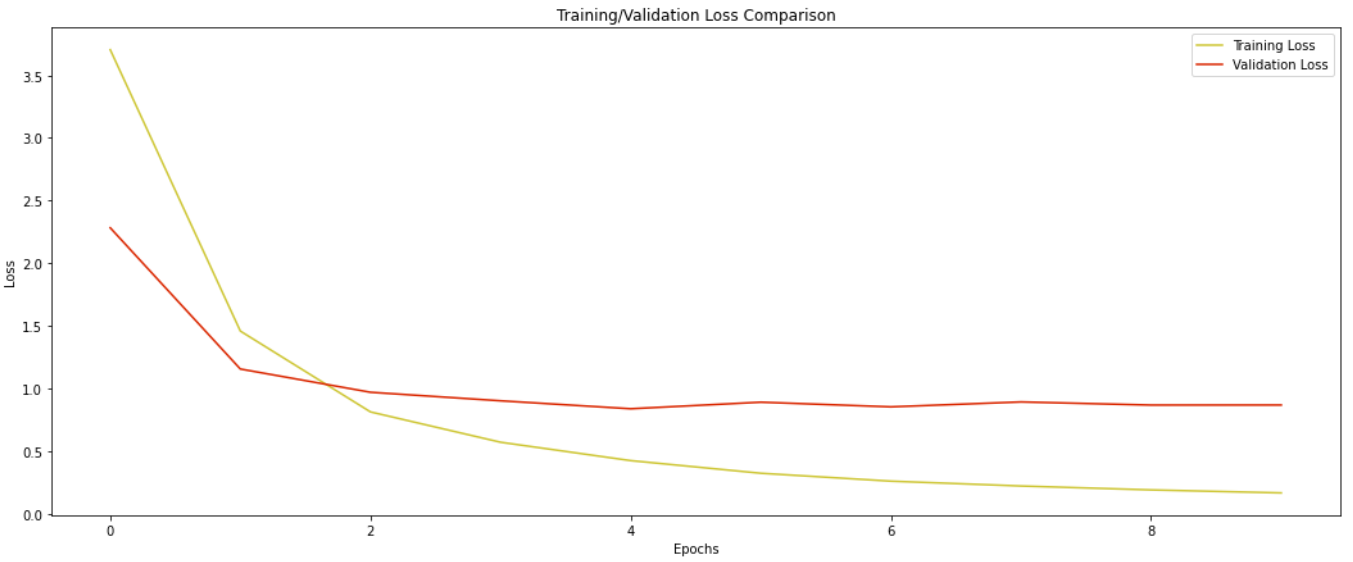
\includegraphics[width=3.5in]{pictures/model1_loss.png}
    \caption{Cross Validation Loss (First Model)}\label{fig:example4}
\end{figure}

\begin{figure}[H]
    \centering
    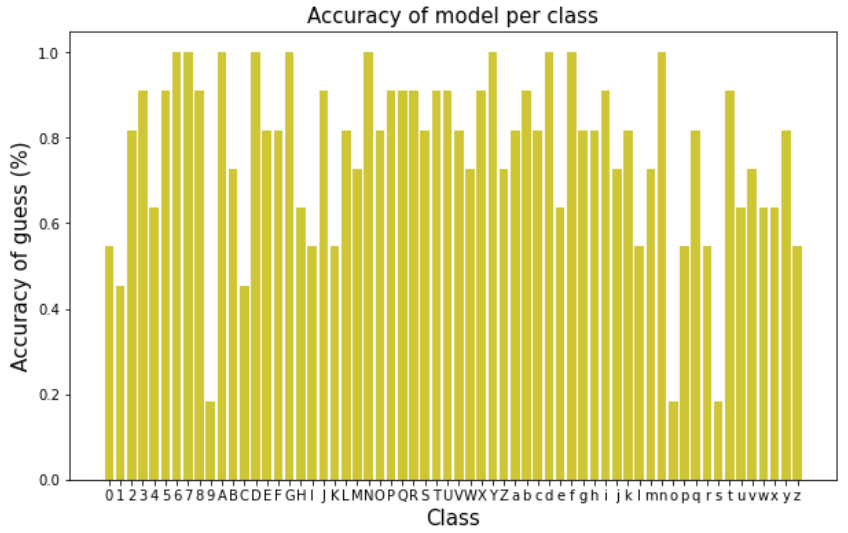
\includegraphics[width=3.5in]{pictures/model1_acc_class.png}
    \caption{Accuracy for each Class (First Model)}\label{fig:example4}
\end{figure}

\begin{figure}[H]
    \centering
    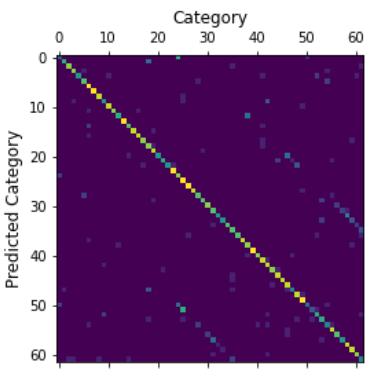
\includegraphics[width=3.5in]{pictures/model2_confmatrix.png}
    \caption{Confusion Matrix (Second Model)}\label{fig:example4}
\end{figure}

\begin{figure}[H]
    \centering
    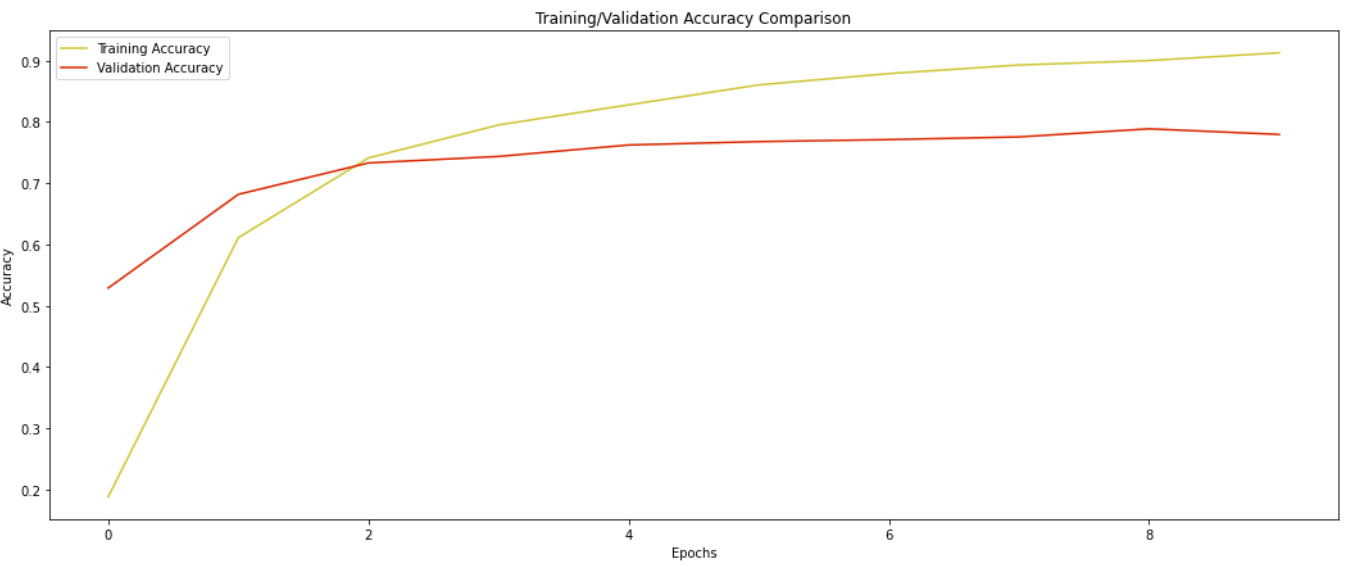
\includegraphics[width=3.5in]{pictures/model2_accuracy.png}
    \caption{Cross Validation Accuracy (Second Model)}\label{fig:example4}
\end{figure}

\begin{figure}[H]
    \centering
    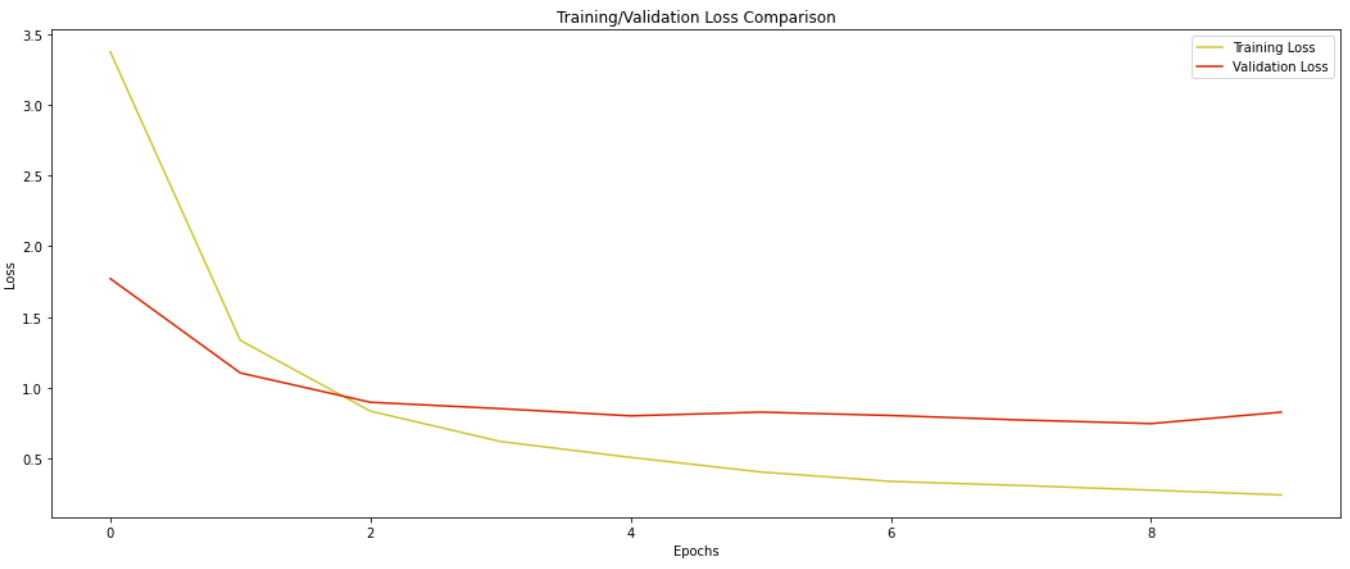
\includegraphics[width=3.5in]{pictures/model2_loss.png}
    \caption{Cross Validation Loss (Second Model)}\label{fig:example4}
\end{figure}

\begin{figure}[H]
    \centering
    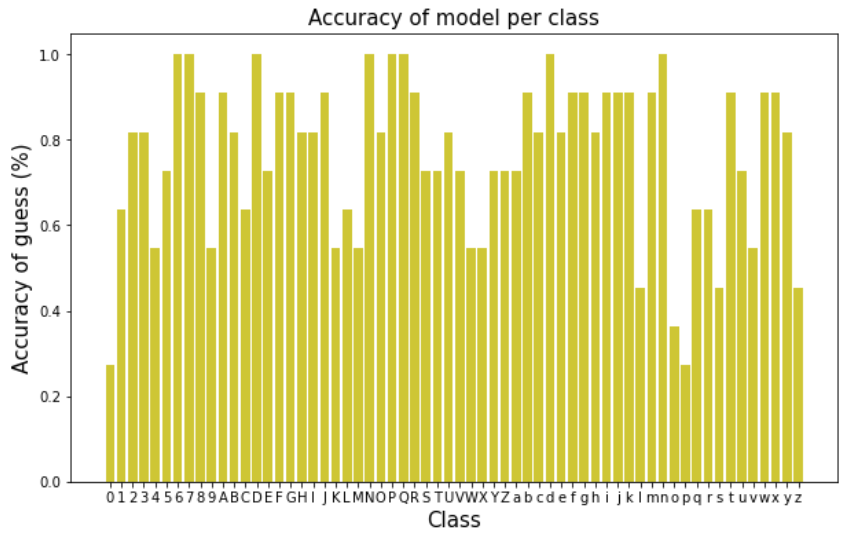
\includegraphics[width=3.5in]{pictures/model2_acc_class.png}
    \caption{Accuracy for each Class (Second Model)}\label{fig:example4}
\end{figure}

In the table below we can compare the 2 algorithms explained in the section above with the techniques we talked about in this section:

\begin{table}[H]
\centering
\caption{Comparison of accuracy and loss of models}
\begin{tabular}{ | m{7em} | m{2.5cm}| m{2.5cm} | } 
\hline
& Model with 3 Convolutional Layers & Model with 2 Convolutional Layers \\ 
\hline
Train Accuracy & 0.9479 & 0.9124 \\
\hline
CV Accuracy & 0.7815249264240265 & 0.7796920835971832 \\
\hline
Test Accuracy & 0.7653958797454834 & 0.7639296054840088 \\
\hline
Train Loss & 0.1544 & 0.2390 \\
\hline
CV Loss & 0.8673150539398193 & 0.8269262760877609 \\
\hline
Test Loss & 0.9538436532020569 & 0.9568818807601929 \\
\hline
\end{tabular}
\end{table}

As we can see in the table above our 2 models managed to obtain similar results.

\section{Hyper-parameters selection}
In previous sections we saw ways of optimizing our model, for instance, having a complete data set as well as pre-processing data the correct way. Here we discuss topics related to hyperparameters that are associated with the values used in the models. These values are key to get good results and must be chosen the correct way. In the next sections we will talk individually about each on of them, what they are, and how we come up to that value. 

\subsection{Learning rates}
In order to address this topic we should start by understanding what is a learning rate. In this article \cite{D} we can see the following :
"Learning rate is a hyper-parameter that controls how much we are adjusting the weights of our network with respect the loss gradient."
Getting a good learning rate is crucial for the proper functioning of the model. Learning rate should not be a hyper parameter chosen naively, therefore there are methods to obtain an appropriate value. For the method we used, we started by defining a very low learning rate and train the model with this value and in the next iterations learning rate exponentially grows according to the following equation:
\linebreak

\begin{equation*}
  f(x) = 0,000125 * 2^x , x\geqslant0
\end{equation*}

However the learning rate cannot increase exponentially forever. It must exist a limit where it stops, because the higher the learning rate does not necessarily mean that model obtains better results. In order to define this value, we researched and came to the conclusion that it might be better to not limit the learning rate but the loss it generates. When getting to a certain value of loss, it means that increasing learning rate will only make it worse, and so the optimal learning rate has already been found.

Below we can see the results we obtained when trying to determine the learning rate to use on our models.

In the first model, that is the one that has 3 Convolutional Layers:
\begin{figure}[H]
    \centering
    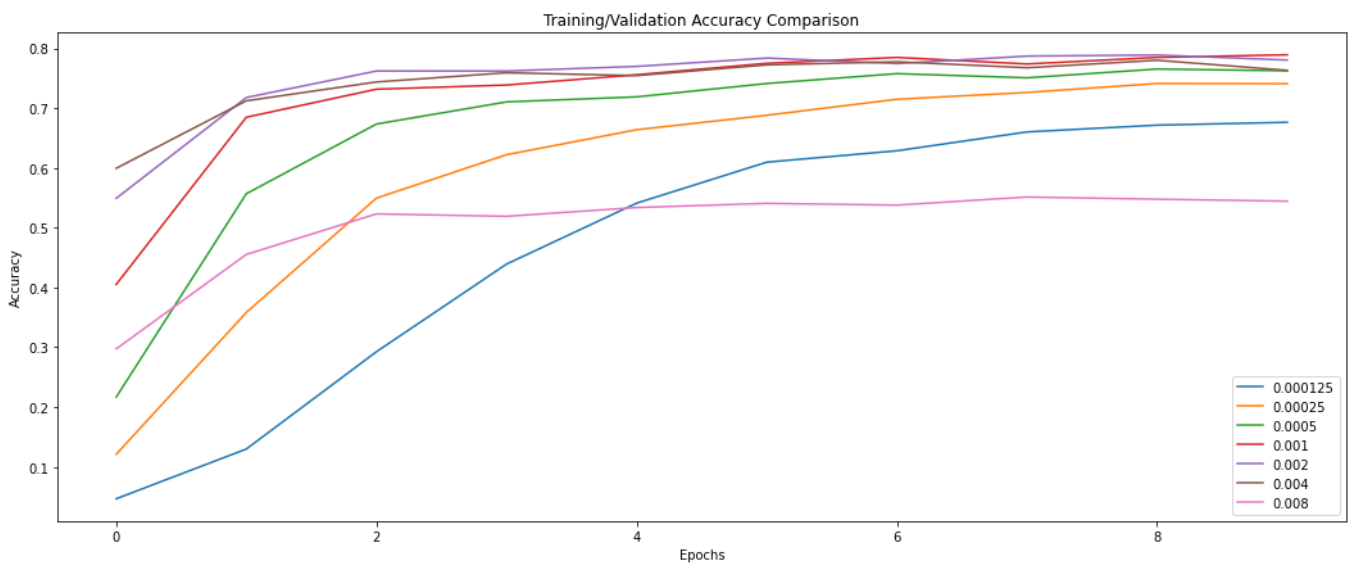
\includegraphics[width=3.5in]{pictures/model1_learning_rate_accuracy.png}
    \caption{Learning rate results on cross Validation Accuracy (First Model)}\label{fig:example4}
\end{figure}

\begin{figure}[H]
    \centering
    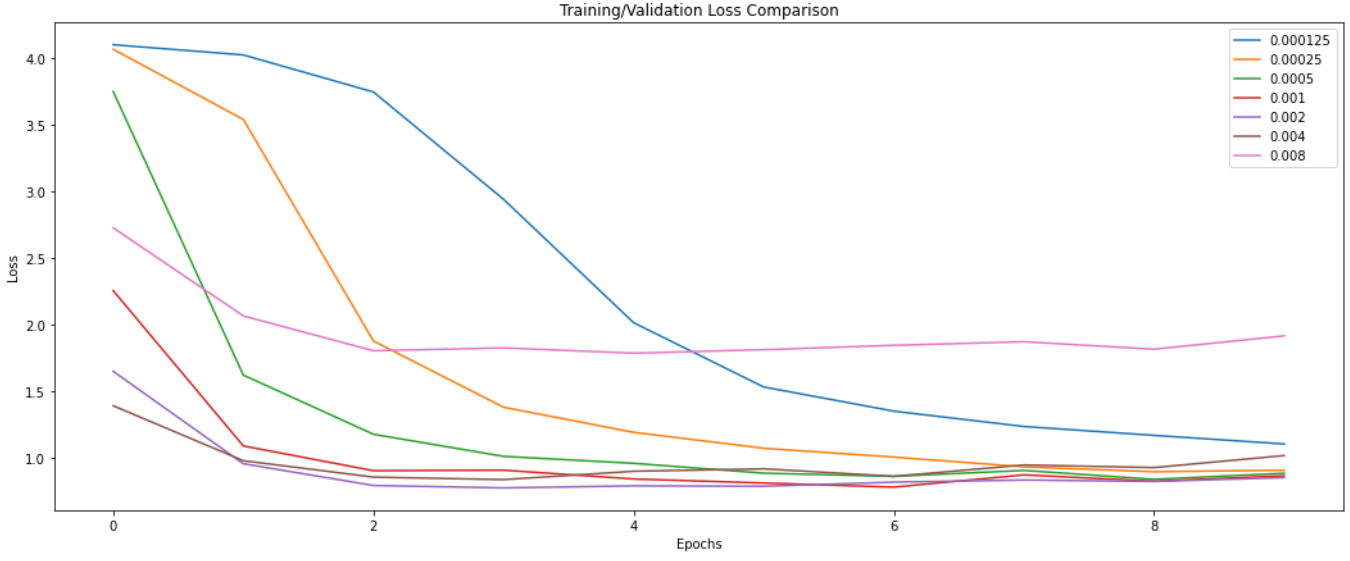
\includegraphics[width=3.5in]{pictures/model1_learning_rate_loss.png}
    \caption{Learning rate results on cross Validation Loss (First Model)}\label{fig:example4}
\end{figure}

\begin{table}[H]
\centering
\caption{Learning rate results on model with 3 Convolutional Layers}
\begin{tabular}{ | m{3.5em} | m{3.2cm}| m{3.2cm} | }
\hline
Learning rate & CV Accuracy & CV Loss \\ 
\hline
0.000125 & 0.6763196438550949 & 1.104457899928093 \\
\hline
0.00025 & 0.7408357858657837 & 0.9080282300710678 \\
\hline
0.0005 & 0.7624633312225342 & 0.884848490357399 \\
\hline
0.001 & 0.7892228662967682 & 0.865957498550415 \\
\hline
0.002 & 0.7804252207279205 & 0.8522607386112213 \\
\hline
0.004 & 0.7631964683532715 & 1.0173208266496658 \\
\hline
0.008 & 0.5443548299372196 & 1.9147809594869614 \\
\hline
\end{tabular}
\end{table}

We can conclude that for this the learning rate that provides better accuracy is 0.001, and being also the second best in the loss, it was the learning rate we decided to use.

In the second model, that is the one that has 2 Convolutional Layers:
\begin{figure}[H]
    \centering
    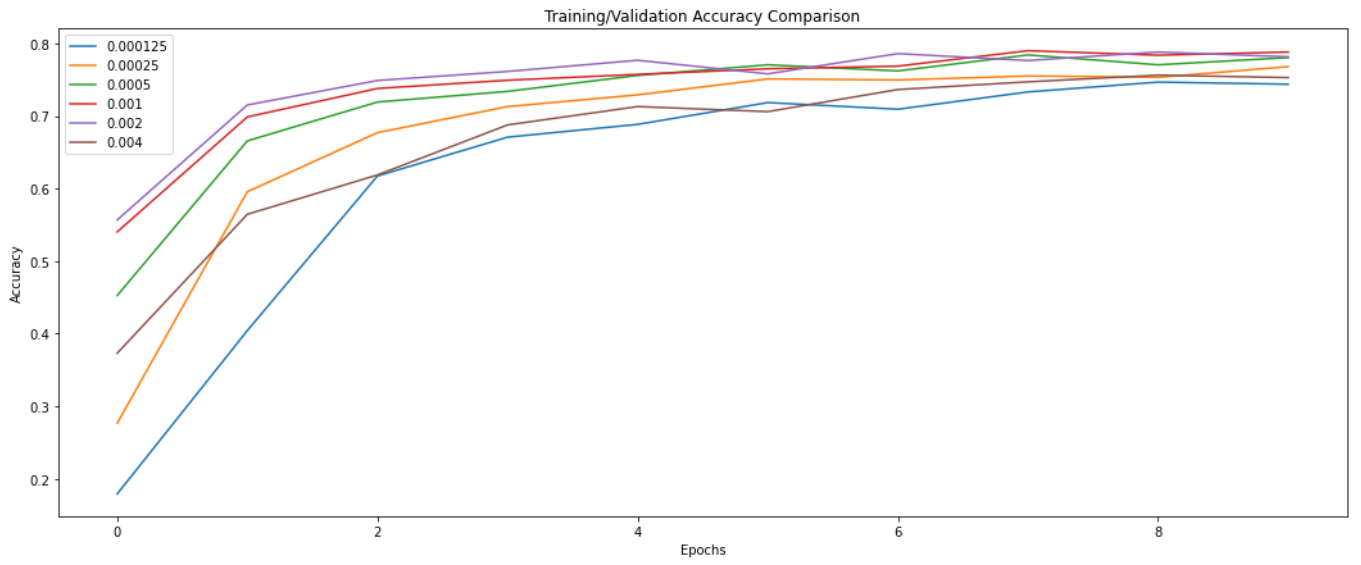
\includegraphics[width=3.5in]{pictures/learning_rate_accuracy.png}
    \caption{Learning rate results on cross Validation Accuracy (Second Model)}\label{fig:example4}
\end{figure}

\begin{figure}[H]
    \centering
    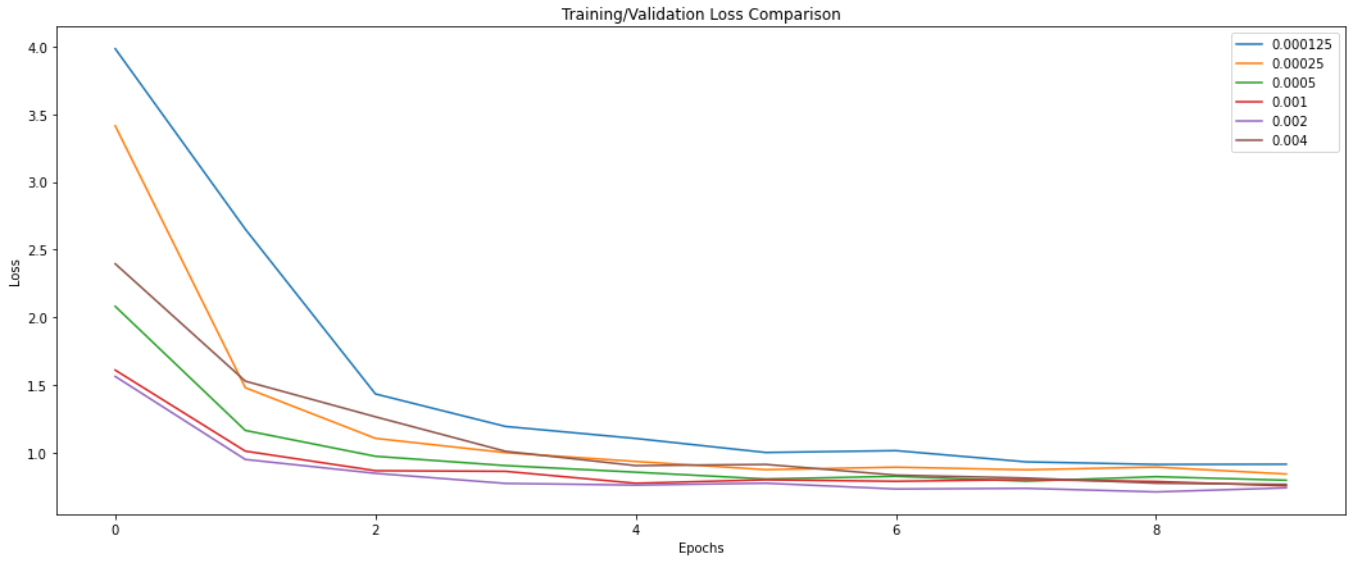
\includegraphics[width=3.5in]{pictures/learning_rate_loss.png}
    \caption{Learning rate results on cross Validation Loss (Second Model)}\label{fig:example4}
\end{figure}

\begin{table}[H]
\centering
\caption{Learning rate results on model with 2 Convolutional Layers}
\begin{tabular}{ | m{3.5em} | m{3.2cm}| m{3.2cm} | } 
\hline
Learning rate & CV Accuracy & CV Loss \\ 
\hline
0.000125 & 0.7437683194875717 & 0.9120788723230362 \\
\hline
0.00025 & 0.7679618746042252 & 0.8397130072116852 \\
\hline
0.0005 & 0.7804252207279205 & 0.7937991768121719 \\
\hline
0.001 & 0.7881231606006622 & 0.7523531913757324 \\
\hline
0.002 & 0.7815249264240265 & 0.7375690042972565 \\
\hline
0.004 & 0.7529325634241104 & 0.7629190683364868 \\
\hline
\end{tabular}
\end{table}

In this model, we got similar results of the learning rate. Just like in the first model, we decided to use a learning rate of 0.001

\subsection{Kernel Size}
The kernel size is a hyper-parameter belonging to the Convolutional Layer. It specifies the window size that the convolutional layer will use to extract features from the image. In other words, if we use a kernel size of 3, the layer's extracting window will be a 3x3 square and it will transform all 9 values into a single one. In order to find the best value for this parameter we decided to start with the value 1 since it cannot be lower than 1 and go up until either the cross-validation loss is way too large or the value just cannot be used given the size of the input.

Using this method of experiment, below we can see the results of kernel size we obtained for each model. In the first model, which has 3 Convolutional Layers these were the results:

\begin{figure}[H]
    \centering
    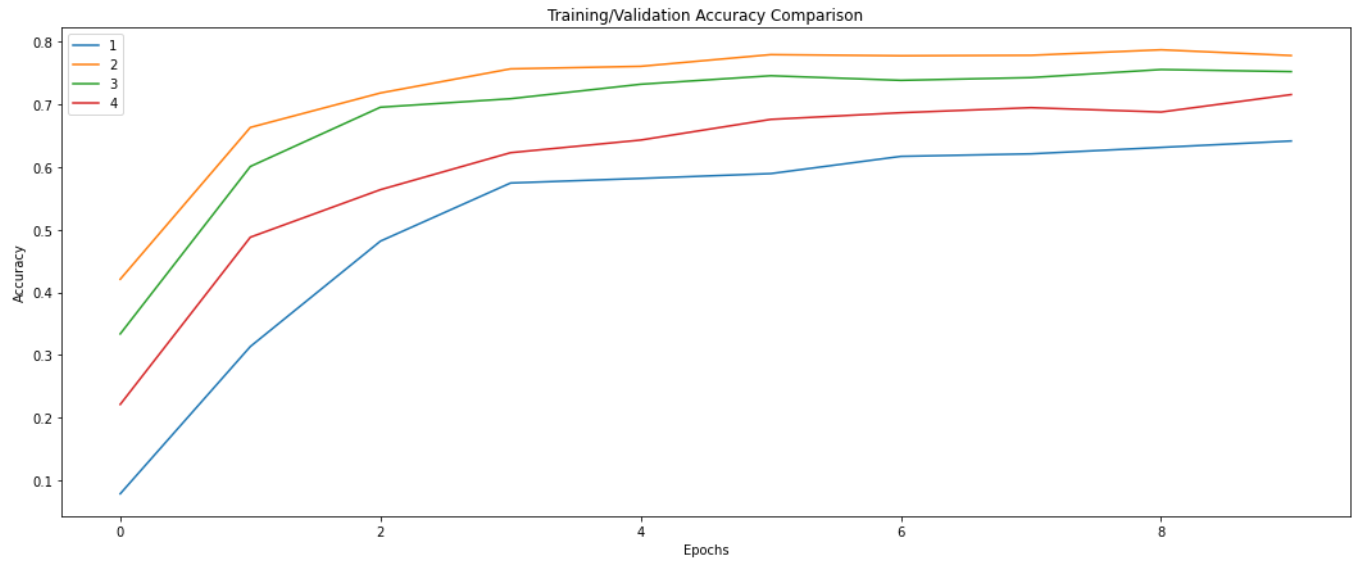
\includegraphics[width=3.5in]{pictures/model1_kernel_size_accuracy.png}
    \caption{Graphic of Kernel size results on cross Validation Accuracy (First Model)}\label{fig:example4}
\end{figure}

\begin{figure}[H]
    \centering
    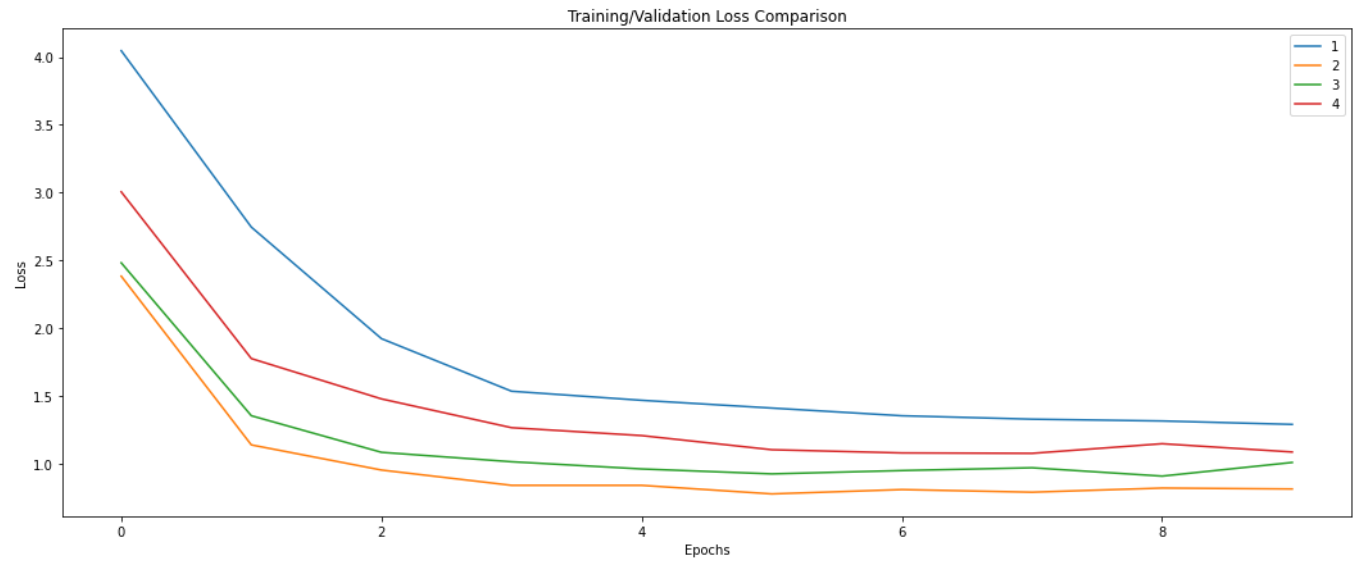
\includegraphics[width=3.5in]{pictures/model1_kernel_size_loss.png}
    \caption{Graphic of Kernel size results on cross Validation Loss (First Model)}\label{fig:example4}
\end{figure}

\begin{table}[H]
\centering
\caption{Kernel size results on model with 3 Convolutional Layers}
\begin{tabular}{ | m{2.5em} | m{3.2cm}| m{3.2cm} | }
\hline
Kernel size & CV Accuracy & CV Loss \\ 
\hline
1 & 0.6414956152439117 & 1.287192702293396 \\
\hline
2 & 0.7778592556715012 & 0.8104611486196518 \\
\hline
3 & 0.7521994113922119 & 1.0061983466148376 \\
\hline
4 & 0.7155425250530243 & 1.0833048224449158 \\
\hline
\end{tabular}
\end{table}

Analyzing these values, we can clearly see that the best kernel size is two, due to providing a better accuracy and has the minor loss function.

In the second model, which has 2 Convolutional Layers, these are the results:

\begin{figure}[H]
    \centering
    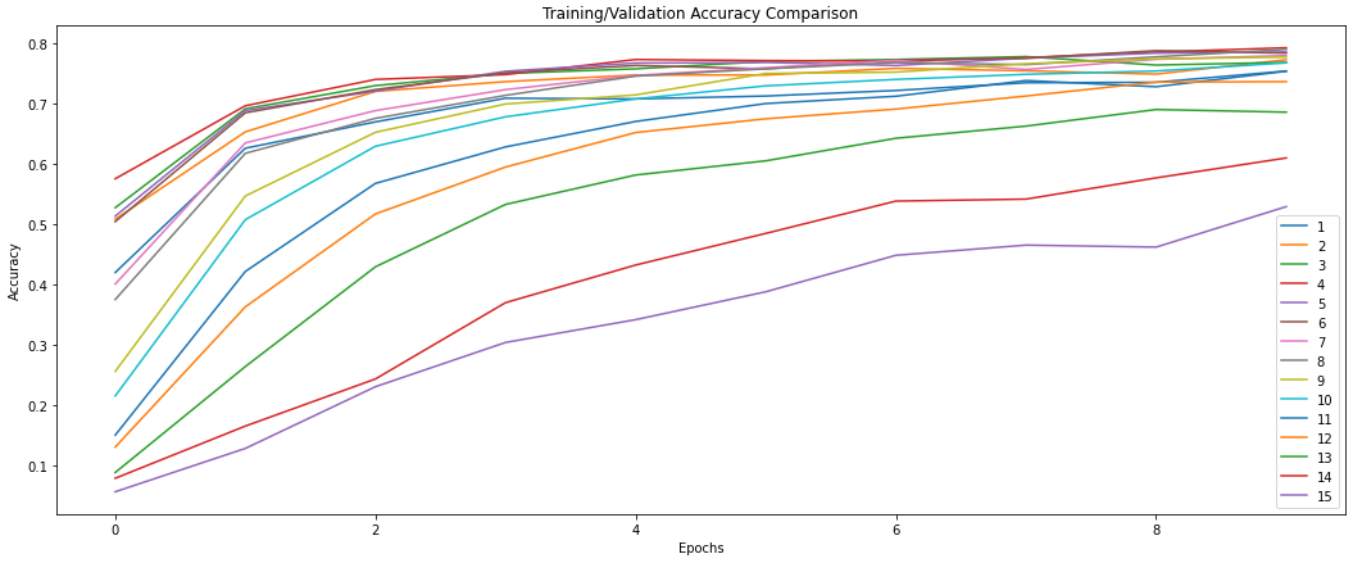
\includegraphics[width=3.5in]{pictures/kernel_size_accuracy.png}
    \caption{Graphic of Kernel size results on cross Validation Accuracy (Second Model)}\label{fig:example4}
\end{figure}

\begin{figure}[H]
    \centering
    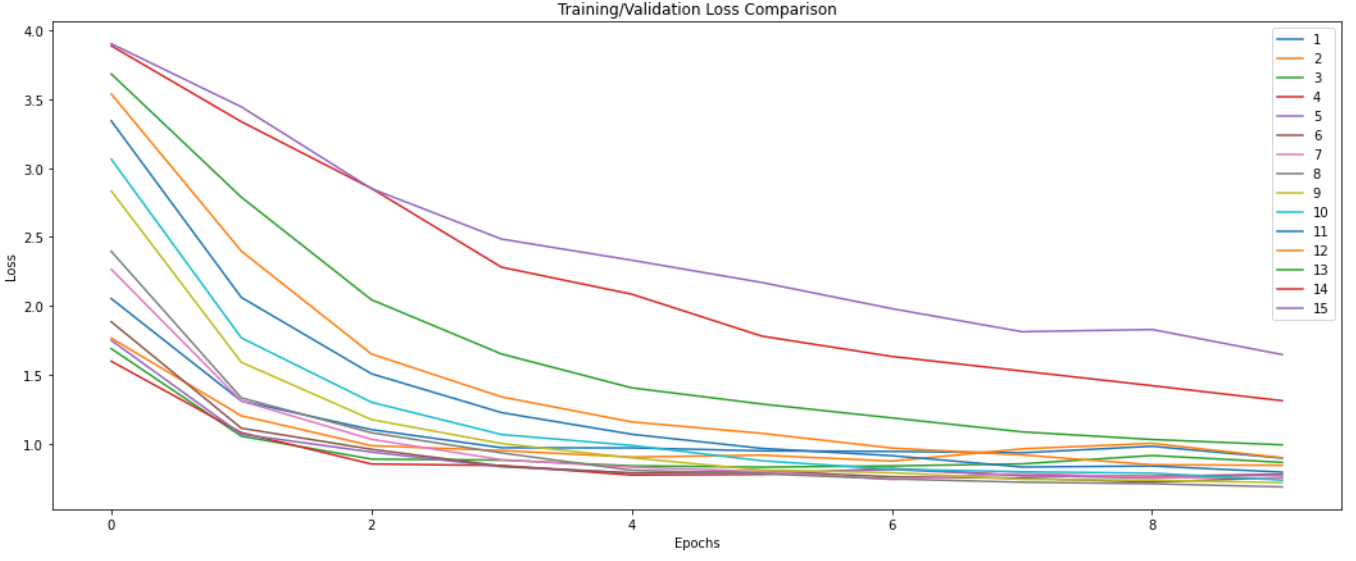
\includegraphics[width=3.5in]{pictures/kernel_size_loss.png}
    \caption{Graphic of Kernel size results on cross Validation Loss (Second Model)}\label{fig:example4}
\end{figure}

\begin{table}[H]
\centering
\caption{Kernel size results on model with 2 Convolutional Layers}
\begin{tabular}{ | m{2.5em} | m{3.2cm}| m{3.2cm} | } 
\hline
Kernel size & CV Accuracy & CV Loss \\ 
\hline
1 & 0.7536657005548477 & 0.893865168094635 \\
\hline
2 & 0.7723607122898102 & 0.8962044417858124 \\
\hline
3 & 0.7679618895053864 & 0.8632470816373825 \\
\hline
4 & 0.7921554148197174 & 0.7759130001068115 \\
\hline
5 & 0.785190612077713 & 0.7760568559169769 \\
\hline
6 & 0.783357784152031 & 0.7536099255084991 \\
\hline
7 & 0.7793255001306534 & 0.750144362449646 \\
\hline
8 & 0.789589449763298 & 0.68498794734478 \\
\hline
9 & 0.776759535074234 & 0.7157995253801346 \\
\hline
10 & 0.7672287225723267 & 0.7345061153173447 \\
\hline
11 & 0.7532991170883179 & 0.7919741272926331 \\
\hline
12 & 0.7360703945159912 & 0.8419033735990524 \\
\hline
13 & 0.6854838728904724 & 0.9902434647083282 \\
\hline
14 & 0.6096041053533554 & 1.3104577660560608 \\
\hline
15 & 0.5289589464664459 & 1.6454468369483948 \\
\hline
\end{tabular}
\end{table}

We can see that in this case the threshold was not reached until the kernel size was sixteen. However like mentioned many times, the bigger this value does not necessarily mean the better. In this case, the kernel size we chosen is four. It is the one that provides a better accuracy as well as providing a small loss in comparison with other values.

\subsection{Dropout Rate \cite{E} \cite{C}}

Dropout is a regularization method where randomly selected nodes are ignored in the model training phase. This nodes are dropped from the model, meaning that they stop contributing to this phase. This regularization method is very interesting and helps in a very common problem in neural networks, which is overfitting.
This is a problem that has not been much addressed in our report, but that is very common to happen. This problem happens when the model produces an high accuracy in the data that is trained, but when it classifies the values of the test set it does not obtain values as good. That is where dropout and other methods like k-fold cross validation come in handy. Dropout helps fight this issue because encourages the model to learn more sparse data, due to the randomly dropped nodes.

To determine dropout rate, we can see in the figure and table below the values we tested and the conclusions we figured out. Once we only used dropout in the second model, there are only graphics related to this model.

\begin{figure}[H]
    \centering
    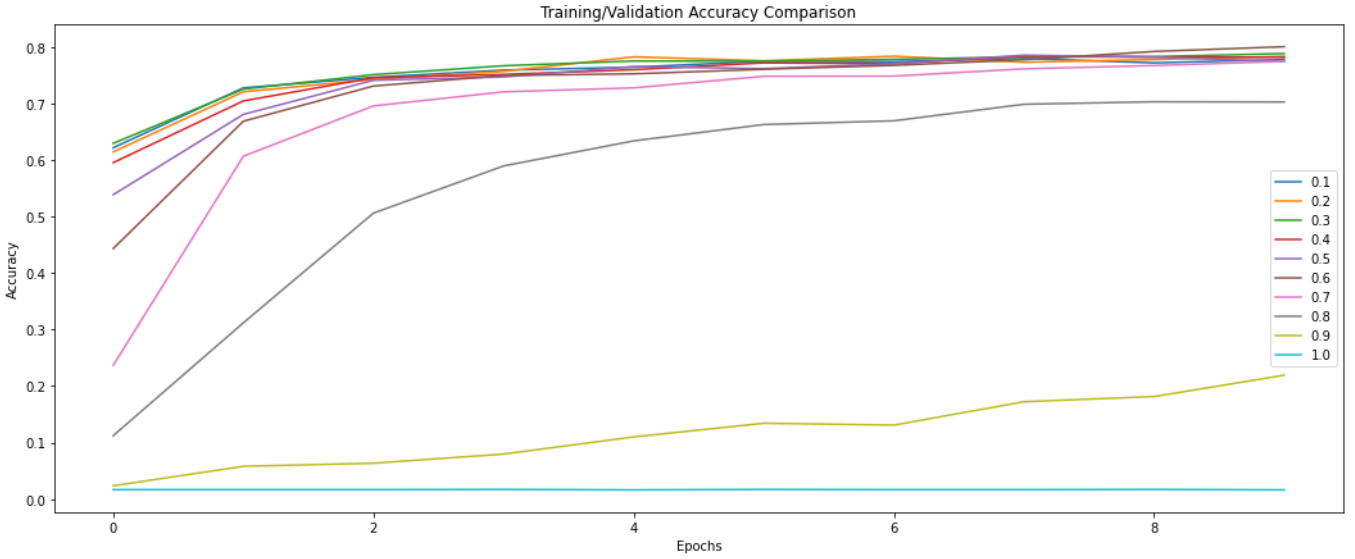
\includegraphics[width=3.5in]{pictures/dropout_rate_accuracy.png}
    \caption{Graphic of Dropout results on cross Validation Accuracy (Second Model)}\label{fig:example4}
\end{figure}

\begin{figure}[H]
    \centering
    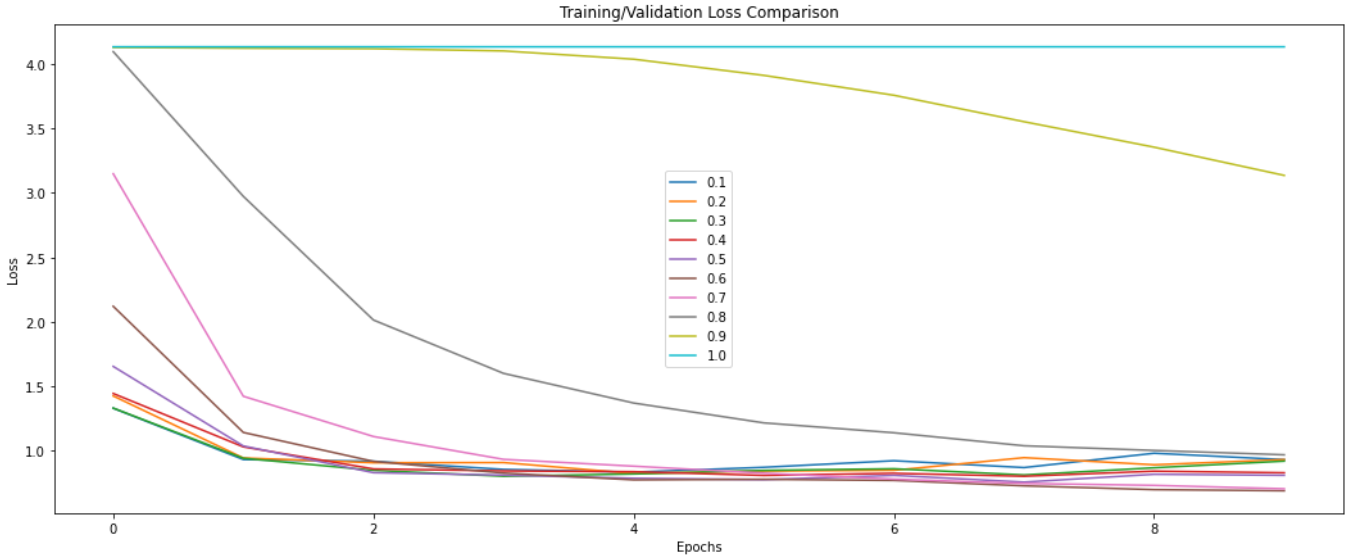
\includegraphics[width=3.5in]{pictures/dropout_rate_loss.png}
    \caption{Graphic of Dropout results on cross Validation Loss (Second Model)}\label{fig:example4}
\end{figure}


\begin{table}[H]
\centering
\caption{Dropout results on model with 2 Convolutional Layers}
\begin{tabular}{ | m{3.5em} | m{3.2cm}| m{3.2cm} | } 
\hline
Dropout rate & CV Accuracy & CV Loss \\ 
\hline
0.1 & 0.7782258093357086 & 0.9330950975418091 \\
\hline
0.2 & 0.7840909063816071 & 0.9334807991981506 \\
\hline
0.3 & 0.7888562977313995 & 0.9214417189359665 \\
\hline
0.4 & 0.782258078455925 & 0.8312205821275711 \\
\hline
0.5 & 0.7745601236820221 & 0.8115196377038956 \\
\hline
0.6 & 0.8009530603885651 & 0.691791221499443 \\
\hline
0.7 & 0.7749266922473907 & 0.7072688788175583 \\
\hline
0.8 & 0.7030791789293289 & 0.9703744798898697 \\
\hline
0.9 & 0.21920821070671082 & 3.1342660784721375 \\
\hline
1.0 & 0.016129032243043184 & 4.130312204360962 \\
\hline
\end{tabular}
\end{table}

Analyzing these values, we came to the conclusion that the best dropout rate to use is 0.6. Putting this value in perspective, a dropout rate of 0.0 is where there are no outputs from the layer, and a dropout of 1.0 is where there is no dropout.

\subsection{Other hyperparameters}
There are other hyper parameters that could be chosen, throughout methods. However due to the lack of computational power to try different values, for instance, a normal computer cannot process high values in the parameter units from the dense layer, as well as high values in the parameter filters from the layer conv2D. Rather than trying different values chosen by methods, we came to the conclusion that it would be more effective to research in articles and algorithms the most commonly used values. This way we decided upon the following values:

\begin{table}[H]
\centering
\caption{Parameters values}
\begin{tabular}{ | m{7em} | m{1cm} | } 
\hline
Hyperparameter & Value\\ 
\hline
Pool-size & 2 \\
\hline
Strides & 2 \\
\hline
Dense units & 512 \\
\hline
Conv2D filters & 32\\
\hline
\end{tabular}
\end{table}

In summary, the choice of hyperparameter values is necessary and must be made strictly. It must be done through methods rather than be chosen through naive approaches. When chosen correctly, these values can drastically improve the accuracy depending on the previously chosen values.

\section{Previous Work}
In this section we plan to compare our work with work that has already been done by other authors. As said previously, our first model is heavily inspired in one found in "kaggle" but we managed to obtain better results after our optimizations. While the author of that model obtained an accuracy around 70 \% we obtained one around 76\%. Unfortunately our data set was only uploaded 2 months ago so there was not a lot of work we could inspire ourselves on. Therefore we tried to study similar work made on other data sets, which allowed us to have a second model with similar results. Although we studied more work, the values in those were obtained in bigger data sets being consequently better. The fact that the data sets are so different makes it difficult to compare those values to ours.

\section{Conclusions}
With this project we managed to create 2 models to recognize handwritten numbers and letters. We believe it was possible to get better results. For example, we had only 55 images of each class which compared to the data sets used in our research is a small number. Also, looking at some images in our data set there were some that we as humans had an hard time guessing, some because they were incomprehensible and others because they were resembled another one, especially some capital and corresponding lowercase letters. Another limitation we faced was the lack of computing power to test some of the parameters (as referred in the previous section) and also to test more complex models.
\linebreak
\tab Through this report we analysed the pre-processing of the data and how it impacts the neural network, we discussed 2 models of deep neural networks and how to train and optimize them. We also seen how a neural network can help in real life situations, especially recognizing a hand written letter or number.



%------- CITATIONS ----------
\nocite{}
\bibliography{references}
\bibliographystyle{IEEEtran}

\nocite{B}
\nocite{A}
\nocite{D}
\nocite{F}
\nocite{C}
\nocite{H}
\nocite{E}
\nocite{G}
\nocite{I}
\nocite{J}
\nocite{K}
\nocite{L}
\nocite{N}
\nocite{O}
\nocite{P}
\nocite{Q}
\nocite{R}
\nocite{S}
\nocite{T}

\section{Division of Work}
In order to complete this project we were most of the time together through zoom, having both students contributed an equal amount of work to its development.
\begin{flushleft}
- Pedro Amaral 50\%
\end{flushleft}
- Ricardo Cruz 50\%

\end{document}


